\section{Span and Rank}

\begin{frame}{Span}
    \begin{itemize}
        \item \textbf{Definition}: The \textbf{span} of a set of vectors $\{\vec{v}_1, \vec{v}_2, \vec{v}_3, \dots\}$ is the set of \textit{all possible linear combinations} of the vectors.
        \item The span of a collection of vectors is always a \textbf{vector space}
        \item Since the column space of a matrix A is the \textit{span of its columns}, it is a vector space.
    \end{itemize}
    \begin{center}
        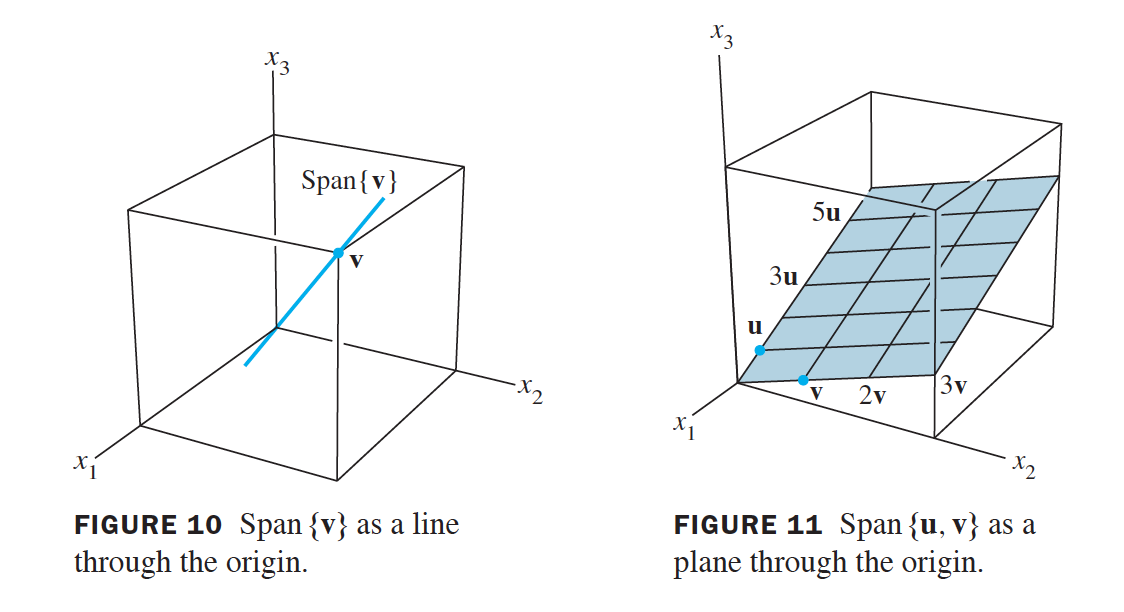
\includegraphics[width = 0.45\textwidth]{images/span1.png}
        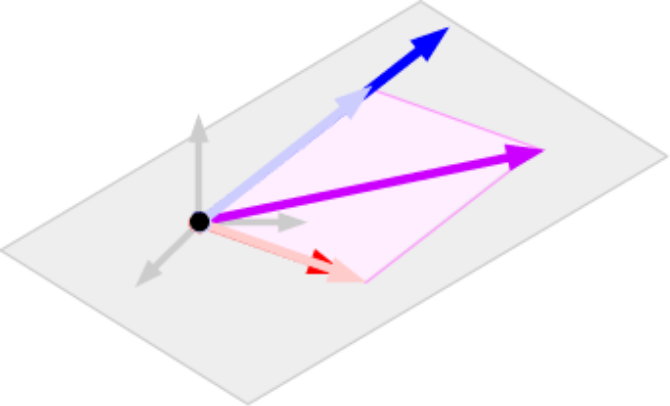
\includegraphics[width = 0.45\textwidth]{images/span2.png}
    \end{center}
\end{frame}

\begin{frame}{Practice: Span}
    Do the following sets of vectors span $\mathbb{R}^3$?
    \begin{align*}
        \bigg\{
            \begin{bmatrix} -1 \\ 0 \\ -1 \end{bmatrix},
            \begin{bmatrix} 1 \\ 0 \\ 1 \end{bmatrix},
            \begin{bmatrix} 1 \\ 1 \\ 1 \end{bmatrix} 
        \bigg\} \\
        \bigg\{
            \begin{bmatrix} -1 \\ 0 \\ 0 \end{bmatrix},
            \begin{bmatrix} 1 \\ 0 \\ 1 \end{bmatrix},
            \begin{bmatrix} 1 \\ 1 \\ 1 \end{bmatrix} 
        \bigg\}
    \end{align*}
\end{frame}

\begin{frame}{Practice: Span [Solution]}
    \begin{align*}
        \bigg\{
            \begin{bmatrix} -1 \\ 0 \\ -1 \end{bmatrix},
            \begin{bmatrix} 1 \\ 0 \\ 1 \end{bmatrix},
            \begin{bmatrix} 1 \\ 1 \\ 1 \end{bmatrix} 
        \bigg\} \Longrightarrow \text{No}\\
        \bigg\{
            \begin{bmatrix} -1 \\ 0 \\ 0 \end{bmatrix},
            \begin{bmatrix} 1 \\ 0 \\ 1 \end{bmatrix},
            \begin{bmatrix} 1 \\ 1 \\ 1 \end{bmatrix} 
        \bigg\} \Longrightarrow \text{Yes}
    \end{align*}
    How do you know if a set of vectors spans $\mathbb{R}^3$?
    \begin{itemize}
        \item Are there \textbf{n pivots}, i.e. \textbf{n linearly independent vectors}?
        \item Use \textit{Gaussian Elimination}!
    \end{itemize}
\end{frame}

\begin{frame}{Rank}
    \begin{itemize}
        \item Definition: The \textbf{rank} of a matrix A is the \textit{dimension of the column space of A}.
        \item Altenatively:
        \begin{itemize}
            \item The number of rows with \textit{nonzero leading coefficients}
            \item The number of \textit{linearly independent columns}.
        \end{itemize}
        \item A \textbf{pivot} is the first nonzero element of a row for a matrix in \textit{row echelon form}, and a pivot column is a column that contains a pivot.
        \item In fact, pivots are shared by both the columns and the rows, so \textbf{dim(colspace($A$)) = dim (rowspace($A$))}.
        \item \textbf{rank($A$) = rank($A^T$)}
    \end{itemize}
\end{frame}

\begin{frame}{Practice: Rank}
    Find the rank of B:
    \begin{align*}
        B = \begin{bmatrix}
            1 & 2 & 1 & -4 \\
            0 & -1 & 1 & -2 \\
            1 &  4 & 1 & 2 \\
        \end{bmatrix}
    \end{align*}
\end{frame}

\begin{frame}{Practice: Rank [Solution]}
    Do Gaussian Elimination!
    \begin{align*}
        \begin{bmatrix}
            1 & 2 & 1 & -4 \\
            0 & -1 & 1 & -2 \\
            1 &  4 & 1 & 2 \\
        \end{bmatrix} \xrightarrow[]{R_3 - R_1 \to R_3}
        \begin{bmatrix}
            1 & 2 & 1 & -4 \\
            0 & -1 & 1 & -2 \\
            0 &  2 & 0 & 6 \\
        \end{bmatrix} \\[1ex]
        \begin{bmatrix}
            1 & 2 & 1 & -4 \\
            0 & -1 & 1 & -2 \\
            0 &  2 & 0 & 6 \\
        \end{bmatrix} \xrightarrow[R_2 \to R_3]{R_3 / 2 \to R_2}
        \begin{bmatrix}
            1 & 2 & 1 & -4 \\
            0 &  1 & 0 & 3 \\
            0 & -1 & 1 & -2 \\
        \end{bmatrix} \\[1ex]
        \begin{bmatrix}
            1 & 2 & 1 & -4 \\
            0 &  1 & 0 & 3 \\
            0 & -1 & 1 & -2 \\
        \end{bmatrix} \xrightarrow[]{R_3 + R_2 \to R_3}
        \begin{bmatrix}
            \boxed{1} & 2 & 1 & -4 \\
            0 &  \boxed{1} & 0 & 3 \\
            0 & 0 & \boxed{1} & 1 \\
        \end{bmatrix}
    \end{align*}
    There are \textit{3 pivot columns}, so \textbf{rank($B$) = 3}.
\end{frame}